% =========================================================================
% CITS4403 Computational Modelling -- Research Project Report
%
% Build with:   make            (output: build/report.pdf)
% Live rebuild: make watch
% Clean up:     make clean
%
% Requirements from the unit specification (RUBICS.md):
%   * maximum five A4 pages, excluding figures, references and appendices
%   * 11pt font and 1-inch margins on all sides
% =========================================================================
\documentclass[11pt,a4paper]{article}

% --- Page layout: 11pt font with 1-inch margins (unit requirement) --------
\usepackage[a4paper,margin=1in]{geometry}

% --- Encoding and fonts ---------------------------------------------------
\usepackage[T1]{fontenc}
\usepackage[utf8]{inputenc}
\usepackage{lmodern}
\usepackage{microtype}
\setlength{\emergencystretch}{1em}

% --- Mathematics ----------------------------------------------------------
\usepackage{amsmath}
\usepackage{amssymb}

% --- Figures, tables and captions -----------------------------------------
\usepackage{graphicx}
\usepackage{booktabs}
\usepackage{caption}
\usepackage{subcaption}

% --- References (BibTeX) --------------------------------------------------
\usepackage[round]{natbib}

% --- Hyperlinks (kept near the end of the preamble) -----------------------
\usepackage[hidelinks]{hyperref}

% --- Title metadata -------------------------------------------------------
\title{Robustness, Cascades and Bus Recovery\\in the Transperth Network}
\author{CITS4403 Project Team\\[2pt]
        \small CITS4403 Computational Modelling, The University of Western Australia}
\date{8 October 2026}
% Generated by report/generate_figures.py from frozen results; do not edit.
\newcommand{\RandomCrossPercent}{6.32}
\newcommand{\DegreeCrossPercent}{1.68}
\newcommand{\BetweenCrossPercent}{1.24}
\newcommand{\CapacityAlphaStar}{0.525}
\newcommand{\EqualAlphaStar}{0.625}
\newcommand{\CoarseAlphaStar}{0.600}
\newcommand{\DemandAlphaStar}{0.750}
\newcommand{\MaxLoadFailed}{86}
\newcommand{\MaxLoadRounds}{31}
\newcommand{\BayRailServicePercent}{67.00}
\newcommand{\BayBusServicePercent}{100.00}
\newcommand{\FremantleRailRatio}{0.68}
\newcommand{\FremantleBusRatio}{1.31}
\newcommand{\AirportRailServicePercent}{93.11}
\newcommand{\AirportBusServicePercent}{66.68}
\newcommand{\AirportRailDemandPercent}{94.50}
\newcommand{\AirportBusDemandPercent}{69.65}
\newcommand{\RecommendedSeeds}{1000}
\newcommand{\WorstHalfWidth}{0.0220}
\newcommand{\WorstMeanChange}{0.0030}
\newcommand{\TailPValue}{0.002}


\begin{document}

\maketitle
\thispagestyle{empty}

\begin{abstract}
\normalsize
\noindent
We model robustness, overload cascades and bus recovery on an audited
86-station Transperth railway. Targeted removal fragments the network sooner
than random station loss. Local load redistribution produces abrupt secondary
failure, whereas shortest-path recomputation on the rail tree contains overload
by dropping unreachable journeys. Bus links can restore service while increasing
rail failures; with a two-link policy after an Airport Line closure, served
terminal pairs fall from \AirportRailServicePercent\% to
\AirportBusServicePercent\%. Sampling and grid checks qualify the thresholds;
the finite avalanche samples do not support a power-law claim.
These findings concern specified routing and capacity proxies, rather than
measured passenger behaviour or operational deployment advice.
\end{abstract}

% Rubric: Background and Research Aims + Originality and Contribution.
% Establish the problem and its significance, state a focused research
% question or modelling objective, position the work against the literature,
% and clearly separate the team's contribution from existing or taught models.

\section{Introduction}
\label{sec:introduction}

\subsection{Background and research aims}
A station closure can sever a railway corridor before any further facility
fails. Substitute buses may reconnect journeys, but the paths they restore can
also concentrate traffic at surviving rail facilities. We investigate these
competing effects in the Transperth network: infrastructure connectivity,
secondary overload failures and the fraction of terminal pairs that remain
served. Fewer open rail facilities need not imply less service when another
transport layer is available.

\citet{albert2000error} established the distinction between random errors and
targeted removal in heterogeneous networks. Their results motivate the
random-versus-targeted comparison here; they do not establish that Transperth
shares their degree distribution or resilience. Our audited railway
has 86 mapped stations and 85 adjacent segments and is a tree, so it lacks
alternative rail paths around a removed station. Its inputs represent
Monday 5 October 2026, 07:00--09:00 in Australia/Perth, with 271 selected rail
trips and 4,324 selected bus trips. These are scheduled services, not measured
passenger journeys. Showgrounds remains a mapped station although it has no
weekday stop event in this window.

\citet{motter2002cascade} showed how a local attack can cause further overload
failures when shortest-path loads are recomputed against capacities fixed from
the intact network. We use that capacity construction and compare it with local
redistribution, in which a failed facility forwards its carried load to
survivors; the comparison tests whether an apparent tolerance transition
depends on the update mechanism. In the bus layer, restored paths
can increase surviving rail loads even while improving terminal reachability.
Apparent avalanche scaling requires a separate statistical test: following
\citet{clauset2009power}, a visual slope alone is not evidence for a power law.

Our research questions are: \textbf{RQ1}, how do random and targeted removal
fragment the railway, and which station characteristics identify bottlenecks?
\textbf{RQ2}, how do capacity tolerance and load-update rules affect the size
and duration of secondary failures? \textbf{RQ3}, when do bus backup links
improve served travel, and can their rerouting aggravate a rail cascade?
\textbf{RQ4}, how sensitive are these conclusions to sampling, tolerance-grid
resolution and the assumed load/capacity model, and is avalanche scaling
statistically supported?

\subsection{Contribution}
Our contribution is a reproducible transport case study that joins an audited
GTFS-derived topology to removal, overload and recovery experiments. We expand
express-service traversals over mapped adjacent segments rather than treating
skipped stops as shortcuts. We separate persistent passenger terminals from
closable rail facilities, retain evidence for substitute links, and compare
infrastructure damage with service outcomes. Paired scenarios and bootstrap
intervals expose uncertainty without treating scheduled departures as observed
demand. The capacity law and robustness questions come from existing work;
the audited Transperth construction, explicit comparison of load-update
assumptions, and evidence-linked recovery analysis are the team's extension.
The implementation is network simulation; the unit's taught agent-based models
are not reused.

% Rubric: Model Specification and Justification.
% Define components, variables, interactions, equations or update rules;
% state assumptions and initialisation; justify model-design and parameter
% choices.

\section{Model specification}
\label{sec:model}

Entity $i$ has state $x_i(t)=(s_i(t),L_i(t))$: open or closed status and carried
load. With neighbours $\mathcal{N}_i$, its generic update is
\begin{equation}
  x_i(t+1) = f\bigl(x_i(t), \{x_j(t)\}_{j \in \mathcal{N}_i}; \theta\bigr),
  \label{eq:update}
\end{equation}
where $\theta$ collects capacities, numerical tolerance and update-mode
parameters. Transport overloads are removed synchronously, then loads are
redistributed or recomputed. The intact-capacity construction follows
\citet{motter2002cascade}; the local variant is specified below. Rounds are
algorithmic, not elapsed time.

\subsection{Components, loads and failure}
The frozen rail layer is an undirected simple tree: 86 stations and 85 adjacent
segments. Multilayer experiments split each station into a
persistent terminal $T{:}i$ and a closable rail facility $R{:}i$ with a
one-minute access edge. Rail edges take
$t_e = \max(0.1,\ d_e/(1000\,v)\cdot 60)$ minutes at an assumed $v = 40$ km/h.
Backup terminal links use four manual effective times (walking, waiting and
transfers) from \texttt{backup\_edges.csv} and GTFS candidates' fastest
scheduled ride times, with no added walking or waiting. Manual rows override
overlapping candidates even when slower, and duplicates within one table keep
the fastest time; the Perth and Perth Underground transfer takes five minutes.
Standby buses activate immediately after the initial closure with unlimited
capacity; multilayer loads are terminal-subset betweenness over the intact
terminal-pair denominator.

The initial load of station $i$ is its unnormalised betweenness on the intact
graph, $L0_i = \sum \sigma_{st}(i) / \sigma_{st}$ over station pairs with
$s \neq i \neq t$, the share of shortest paths through $i$. Unnormalised values
keep rounds comparable as the graph shrinks; normalised loads would rise with
the shrinking node set. The load modes are \texttt{betweenness} as above;
\texttt{betweenness\_freq} with edge length $1/\text{trips}$;
\texttt{betweenness\_plus\_trips} with $0.1\,\text{trips served}_i$ added to
give leaf stations a positive baseline; and \texttt{demand}, the AM-peak
scheduled departure count \texttt{am\_peak\_stops}, a boardings proxy rather
than passenger counts.

Capacities follow
\begin{equation}
  C_i = (1+\alpha) K_i, \qquad \alpha \ge 0,
  \label{eq:capacity}
\end{equation}
with intact reference $K_i = L0_i$ by default, fixed throughout the cascade.
Zero initial load gives zero capacity, but positive static redistribution can
still overload it. For the demand experiment, $L0_i = \text{am\_peak\_stops}_i$,
$f_i = \text{trips\_served}_i$, and $K_i = c f_i$ with
$c = \max_{i:f_i>0}(L0_i/f_i)$. This smallest uniform scale covering demand is
a recorded scenario assumption. Zero frequency with zero demand gives $K_i=0$;
positive demand with zero frequency is rejected.

At each round every surviving station with $L_i > C_i + \delta$ fails, where
the numerical tolerance $\delta$ defaults to $10^{-12}$; the round's overloads
are collected before any removal, and the cascade stops at the first clear
round. The first failure is an explicit \texttt{target} if named, otherwise the
largest initial load (\texttt{load}), the highest degree with station-ID ties
(\texttt{degree}), or a uniform seeded draw (\texttt{random}). A line closure
replaces the trigger with one initial batch, removed before the first check and
excluded from the secondary avalanche size. In the static mode a closed station
forwards its load equally over survivors or in proportion to their capacities,
with equal shares when all have zero; a station with no survivor removes its
load, and otherwise load is conserved. The dynamic mode recomputes loads on the
surviving graph each round and ignores redistribution; on a tree this cannot
raise a survivor's betweenness, so containment reflects dropped journeys rather
than headroom. The containment tolerance $\alpha^*$ is the smallest sampled
$\alpha$ at which the maximum-load trigger causes no secondary failure.

\subsection{Assumptions and initialisation}
All facilities start open; loads and capacities come from the intact graph, and
the trigger or initial batch is applied before the first overload check. The
model assumes undirected adjacent links, scheduled services as load proxies,
hop distances for load concentration, minutes only in the multilayer layer,
symmetric bus times, unlimited immediate standby, and one service date. An
empty initial batch closes nothing; an
$\alpha$ of zero adds no headroom and can fail a station immediately; zero
capacity does not exempt a station from overload checks.

\texttt{src/transperth/config.py} defaults to $\alpha=0.2$, master seed 0,
tolerance $10^{-12}$ and the 81-point grid $\alpha=0,0.025,\ldots,2$.
The tolerance guards floating-point comparisons. The grid starts at zero,
reaches twice the $L0$ reference, and brackets the sampled containment
tolerances near 0.5 and 0.75; its 0.025 step resolves the abrupt static
transition (RQ4).
% Rubric: Experimental Design.
% Specify scenarios, parameter ranges, outcome measures and, where relevant,
% repeated runs and comparisons, with enough detail for the experiments to be
% repeated.

\section{Experimental design}
\label{sec:experiments}

Five runner families produce the evidence, each from one command in the
repository root. They load the frozen graph, apply the model of
Section~\ref{sec:model}, and write their tables and figures under
\texttt{results/} and \texttt{figures/}. Table~\ref{tab:design} lists each
family's scenarios, runner defaults and outcome measures.

\begin{table}[t]
  \centering
  \scriptsize
  \setlength{\tabcolsep}{4pt}
  \caption{Scenarios, runner defaults and outcome measures.}
  \label{tab:design}
  \begin{tabular}{@{}p{0.15\linewidth} p{0.49\linewidth} p{0.33\linewidth}@{}}
    \toprule
    Command & Scenarios and runner defaults & Outcome measures \\
    \midrule
    RQ1: \texttt{make percolation} &
    Random and targeted node and edge removal ranked by degree, betweenness
    and demand flow; fractions 0.00 to 0.90 in 0.01 steps plus 1.00, 100 seeds
    each; every station once as trigger over 81 tolerances ($\alpha = 0$ to
    $2$, step 0.025), static capacity rule &
    Seed-mean GCC fraction and isolates; susceptibility peak; GCC $= 0.5$
    crossing; containment tolerance; predictor strength and rank stability \\
    \addlinespace
    RQ2: \texttt{make cascade} &
    Static sweep $\alpha = 0$ to $2$ in 0.025 steps with \texttt{equal} and
    \texttt{capacity} rules; maximum-load, maximum-degree and 300 seeded
    random triggers. A reduced 10-point grid adds the frequency and demand
    load modes and dynamic rerouting. 2{,}000 random triggers at
    $\alpha = 0.1, 0.15, 0.2, 0.3$; line closures as one batch &
    Failed fraction; avalanche size, duration and span; containment
    $\alpha^*$; paired rule, load-mode and rerouting differences \\
    \addlinespace
    RQ3: \texttt{make recovery} &
    21 closures: 8 exclusive-station lines, 8 interchanges, 5 seeded random
    sets of 5. Five strategies with a 2-link budget over 4 manual and 266
    GTFS-derived candidate pairs; layered cascade $\alpha = 0$ to $2$ in 0.05
    steps; focus checks at 0 and 0.2 &
    Served OD fraction and endpoint-sum demand over 3{,}655 terminal pairs;
    secondary rail closures and recovery rounds; travel-time penalty
    conditional on reachable pairs \\
    \addlinespace
    RQ4: \texttt{make demand} &
    Topology (betweenness loads, $K = L0$) against demand
    (\texttt{am\_peak\_stops} loads, frequency-scaled $K$); 81 tolerances
    from 0 to 2 in 0.025 steps; maximum-load trigger; capacity rule &
    Load and rank changes; Spearman correlation; top-5, top-10 and top-20
    overlap; containment-tolerance shift \\
    \addlinespace
    RQ4: \texttt{make uncertainty} &
    1{,}000 random draws per removal fraction (0 to 1, step 0.05); 95\%
    percentile bootstrap with 2{,}000 resamples; nested seed prefixes 25 to
    2{,}000; alpha grids from 0.5 to 0.025; power-law test with 500 refitted
    simulations at $\alpha = 0.1, 0.15, 0.2, 0.3$ &
    Pointwise interval half widths; seed convergence; grid-induced
    containment shift; tail eligibility and rejection probability \\
    \bottomrule
  \end{tabular}
\end{table}

All runs use master seed 0 and derived child seeds, so paired conditions share
random draws while repeated draws remain separate observations. Each runner
writes one row per replicate through \texttt{experiments.save\_table}, with a
\texttt{.meta.json} sidecar holding the seed, parameters, package versions and
SHA-256 hashes of inputs and code, plus a family manifest that hashes the
artifacts; \texttt{--quick} variants are smoke tests in separate directories.

The pipeline is runner, stored rows, statistics, report. The runners call the
packaged engines and store raw per-seed rows under \texttt{results/<family>/};
the P1.2 helpers summarise them as means and percentile intervals;
\texttt{make figures} checks the tables against their sidecars and manifests,
then writes the report figures and the macros in
\texttt{sections/00-results-values.tex}; and Section~\ref{sec:results} cites
those frozen files. Notebooks 01 to 04 (issues P3.1 to P3.4) re-execute the
same calls interactively. \texttt{make check} runs the test suite and
\texttt{make reproduce} chains \texttt{data}, \texttt{check},
\texttt{figures} and \texttt{notebooks}; each family regenerates with its
command in Table~\ref{tab:design}. \path{run_uncertainty.py} verifies the
committed P2.2 manifest before running, so P2.2 is regenerated first if its
inputs change.
% Rubric: Results.
% Report qualitative and quantitative findings accurately, with well-chosen
% figures and tables that have informative captions, labels and units.
% Save figures to figures/ and include them with \includegraphics, as in the
% commented example below.

\section{Results}
\label{sec:results}

\subsection{RQ1: targeted removal exposes corridor bottlenecks}
Figure~\ref{fig:robustness-cascade}a shows earlier fragmentation under targeted
station removal. The interpolated removal fraction at which the mean largest
component reaches half of the intact 86 stations is
\RandomCrossPercent\% for random removal, \DegreeCrossPercent\% for a fixed
degree ranking and \BetweenCrossPercent\% for a fixed betweenness ranking.
These estimates are distinct from the susceptibility peaks of the
second-largest component at 6\%, 2\% and 1\%, and depend on station-count
rounding and grid resolution; on this small tree, neither diagnostic
establishes a thermodynamic phase transition. Betweenness identifies
corridor-separating positions that degree alone cannot distinguish: many
internal stations have degree two but sit between different amounts of the
network.

\subsection{RQ2: tolerance depends on the load-update assumption}
For the maximum-load trigger, Oats Street, static capacity-weighted
redistribution at $\alpha=0.2$ closes all \MaxLoadFailed{} stations, including
the trigger, in \MaxLoadRounds{} secondary rounds. On the 0.025 grid, the first
sampled tolerance containing the closure is $\alpha=\CapacityAlphaStar$;
equal redistribution requires $\alpha=\EqualAlphaStar$
(Figure~\ref{fig:robustness-cascade}b). These are sampled thresholds for the
specified trigger and rule, not universal station-capacity requirements.
Dynamic unweighted betweenness produces no secondary failures on the frozen
tree (Section~\ref{sec:model}): the disconnected graph can still lose service.
The 2,000 random-trigger observations include zero secondary failures; cascade
rounds are not separate trials. The observed size
distribution is concentrated at a few finite outcomes
(Figure~\ref{fig:uncertainty}b).

\subsection{RQ3: service recovery and rail damage can move in opposite directions}
After a Bayswater closure at $\alpha=0.2$, the rail-only scenario serves
\BayRailServicePercent\% of the original 3,655 terminal pairs. Full candidate
bus standby serves \BayBusServicePercent\%, but closes two rail facilities
instead of one (Figure~\ref{fig:bus-mechanism}a). At the first load check,
Fremantle's load-to-capacity ratio rises from \FremantleRailRatio{} without
buses to \FremantleBusRatio{} with the full pool
(Figure~\ref{fig:bus-mechanism}b), above the fixed rail-only capacity, so it
fails next; bus paths still keep its terminal connected. At $\alpha=1.0$, the
full-pool Bayswater case serves all pairs with only the trigger closed, so
extra capacity can contain the rerouting overload that the restored paths
created.

The complete pool does not worsen served service in the stored scan;
a budgeted strategy can. After the three exclusive Airport Line facilities
close at $\alpha=0.2$, the existing-bus policy selects two links and additionally
closes West Leederville. Served terminal pairs fall from
\AirportRailServicePercent\% with no backup to \AirportBusServicePercent\%.
Endpoint-weighted served demand likewise falls from
\AirportRailDemandPercent\% to \AirportBusDemandPercent\%
(Table~\ref{tab:airport}). These weights sum scheduled stop counts at pair
endpoints, not observed OD demand. Travel-time penalties are conditional on
reachable pairs; comparing means alone could mistake lost long journeys for
faster service.

\subsection{RQ4: numerical uncertainty and model sensitivity}
The tested nested-prefix criteria recommend \RecommendedSeeds{} random trials:
the worst normalised mean change is \WorstMeanChange{} and the largest pointwise
95\% interval half width is \WorstHalfWidth{}, below the chosen 0.02 and 0.03
tolerances (Figure~\ref{fig:uncertainty}a). These criteria apply to the stored
conditions, not every transport model. Coarsening the capacity-rule alpha grid
from 0.025 to 0.1 shifts first sampled containment from
\CapacityAlphaStar{} to \CoarseAlphaStar{}. The demand/frequency-capacity
scenario gives \DemandAlphaStar{}; it changes the load proxy, capacity
reference and trigger, so it is a model comparison, not an isolated demand
effect. Frequency weighting alone leaves unique tree paths unchanged.

The bounded power-law test uses maximum-likelihood fitting, cutoff selection
and refitted simulation, not log-log regression
\citep{clauset2009power}. At static alpha 0.1--0.2 there are only two distinct
positive secondary sizes, making the tail ineligible under the three-size
requirement. At 0.3 the fitted hypothesis is rejected
($p=\TailPValue$, 500 refitted simulations), with its exponent at the lower
search boundary. Dynamic samples contain only zeros. The experiments therefore
do not support a power-law avalanche claim.

% \begin{figure}[t]
%   \centering
%   \includegraphics[width=0.8\linewidth]{figures/example.png}
%   \caption{State what is shown, under which conditions, and the units.}
%   \label{fig:example}
% \end{figure}

% Then refer to Figure~\ref{fig:example} in the discussion of the finding.

% Rubric: Discussion and Conclusions.
% Interpret findings in relation to the research question, draw
% evidence-supported conclusions, and identify limitations, uncertainty and
% potential improvements or applications without overstating the model scope.

\section{Discussion and conclusions}
\label{sec:discussion}

The tree topology explains RQ1's vulnerability: removing a station can cut the
only rail path between corridors, and extra capacity cannot restore a deleted
edge. RQ2 concerns whether surviving facilities acquire further overloads.
Dynamic containment reflects disappearing load, not preserved service; the
static all-station cascade is conditional on the forwarding rule and is not
evidence that a single closure would destroy Perth's railway.

RQ3 shows why recovery needs both service and facility metrics. Backup paths
can reconnect terminals while increasing load at particular rail facilities;
the Fremantle case traces that overload. Enough substitute connectivity can
maintain travel despite the extra closure, while a limited selection can leave
the network worse after secondary failures. Policies should
therefore be compared after the cascade stabilises, with a common intact OD
denominator and the reachable population reported beside travel times. Our
two-link budget counts selected connections, not fleet size.

Uncertainty remains broader than the Monte Carlo intervals in RQ4. We study
one service date and window, mapped undirected links, approximate rail speeds,
proxy capacities, symmetric effective bus times and immediate unlimited bus
standby. The model omits measured boarding/alighting, vehicle occupancy,
directional timetables, congestion, dispatch delay and finite substitute
capacity. Terminal-pair reachability is not proof of a feasible journey, and
the finite 86-station support limits tail inference: rejection cannot establish
the absence of scaling elsewhere.

Next tests would add observed OD demand and vehicle capacity, directional
time-dependent routing, delayed finite bus deployment, and several service-day
snapshots; enumerating all 86 triggers would remove trigger-sampling error. The
conclusions are narrower: targeted corridor removal is structurally damaging;
overload containment depends on the update rule and tolerance grid; and
substitute connectivity can improve service while aggravating rail overload.
These mechanisms are testable against operational evidence.


% Figure pages are excluded from the five-page main-body limit.
\clearpage
\section*{Selected figures}

\begin{figure}[!ht]
  \centering
  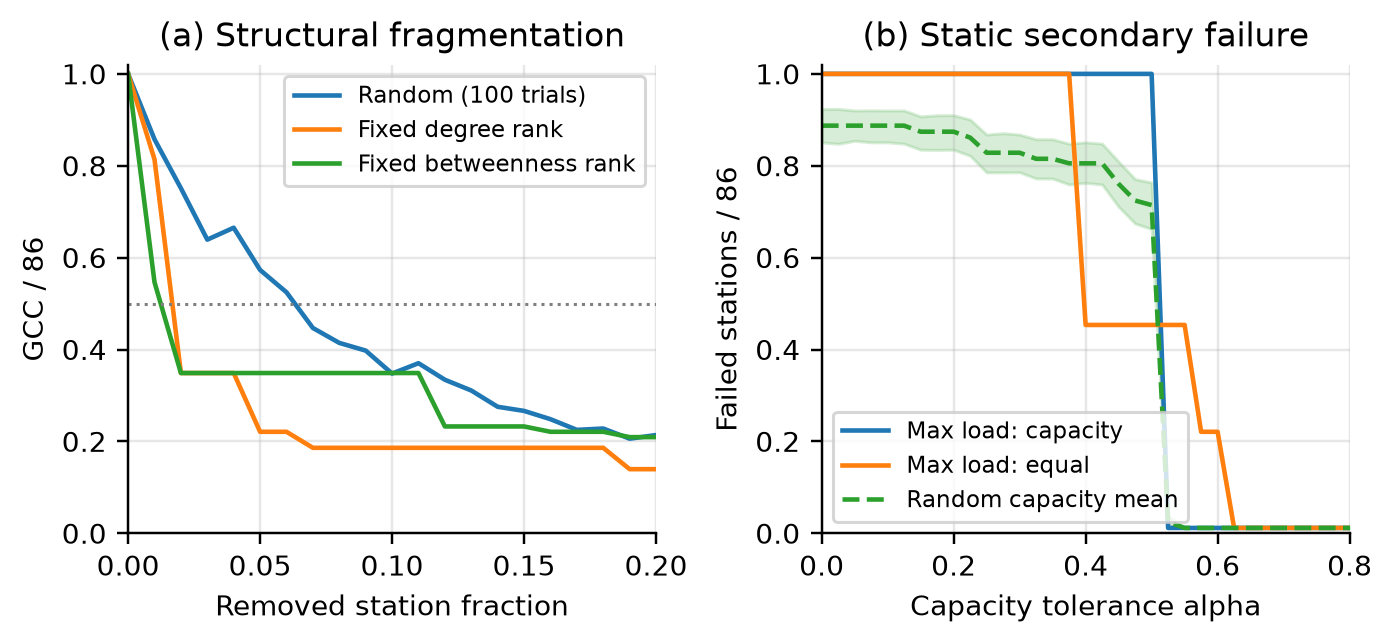
\includegraphics[width=\linewidth]{figures/robustness_cascade.png}
  \caption{Frozen 86-station railway. (a) Station-removal curves, with the
  horizontal GCC/86=0.5 diagnostic. The random mean uses 100 trials per
  fraction; target orders are fixed from the intact graph. (b) Static
  unweighted-betweenness cascades. Targeted curves use the maximum-load station;
  the random capacity-rule mean uses 300 whole trigger trials per alpha and
  pointwise 95\% bootstrap intervals with 2,000 resamples. Failed fractions
  include the trigger. Sources: P2.1 percolation tables, P2.2 runs and P2.5
  cascade intervals; selected by \texttt{report/generate\_figures.py}.}
  \label{fig:robustness-cascade}
\end{figure}

\begin{figure}[!ht]
  \centering
  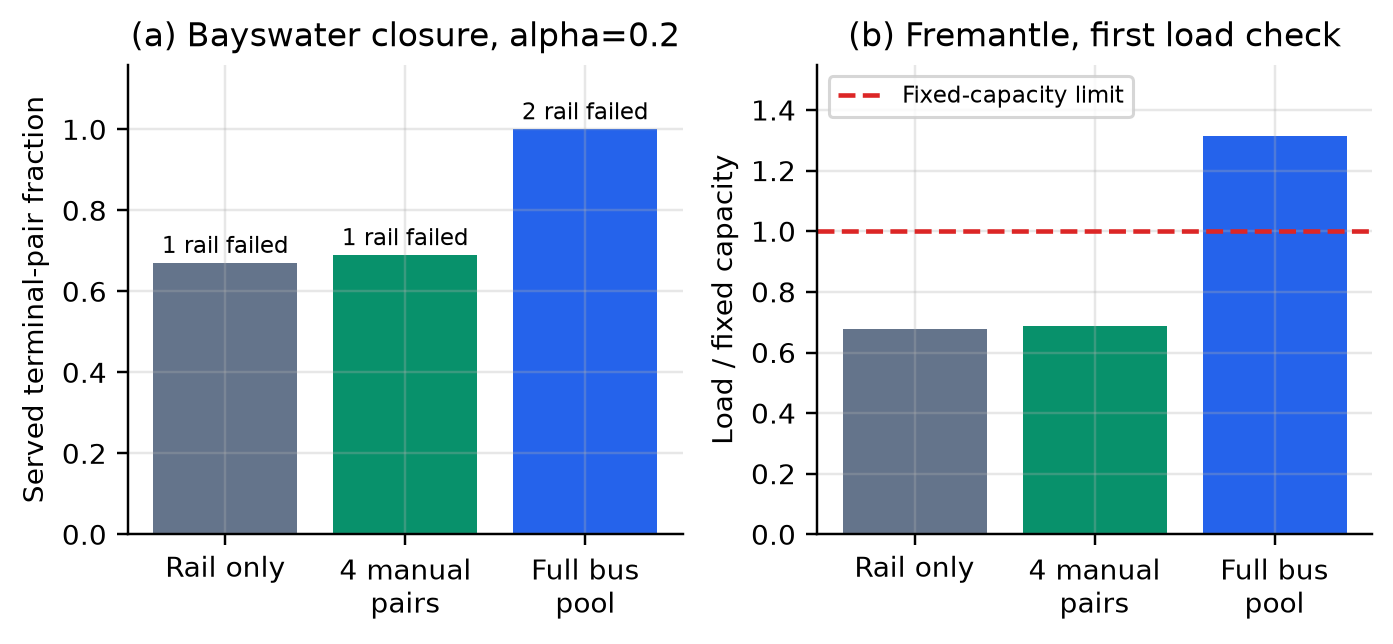
\includegraphics[width=\linewidth]{figures/bus_service_mechanism.png}
  \caption{Bayswater closure at $\alpha=0.2$, layered dynamic routing with
  capacities fixed from the intact rail-only baseline. (a) Served terminal
  pairs over the original 3,655 pairs; annotations count failed rail facilities,
  including the trigger. (b) Fremantle's load/capacity ratio immediately after
  the trigger, before secondary closures. The full bus pool restores all pairs
  while pushing Fremantle above one. This is immediate unlimited standby,
  not a two-link budget. Sources: P2.3 bus-cascade scan and loads tables.}
  \label{fig:bus-mechanism}
\end{figure}

\clearpage
\begin{figure}[!ht]
  \centering
  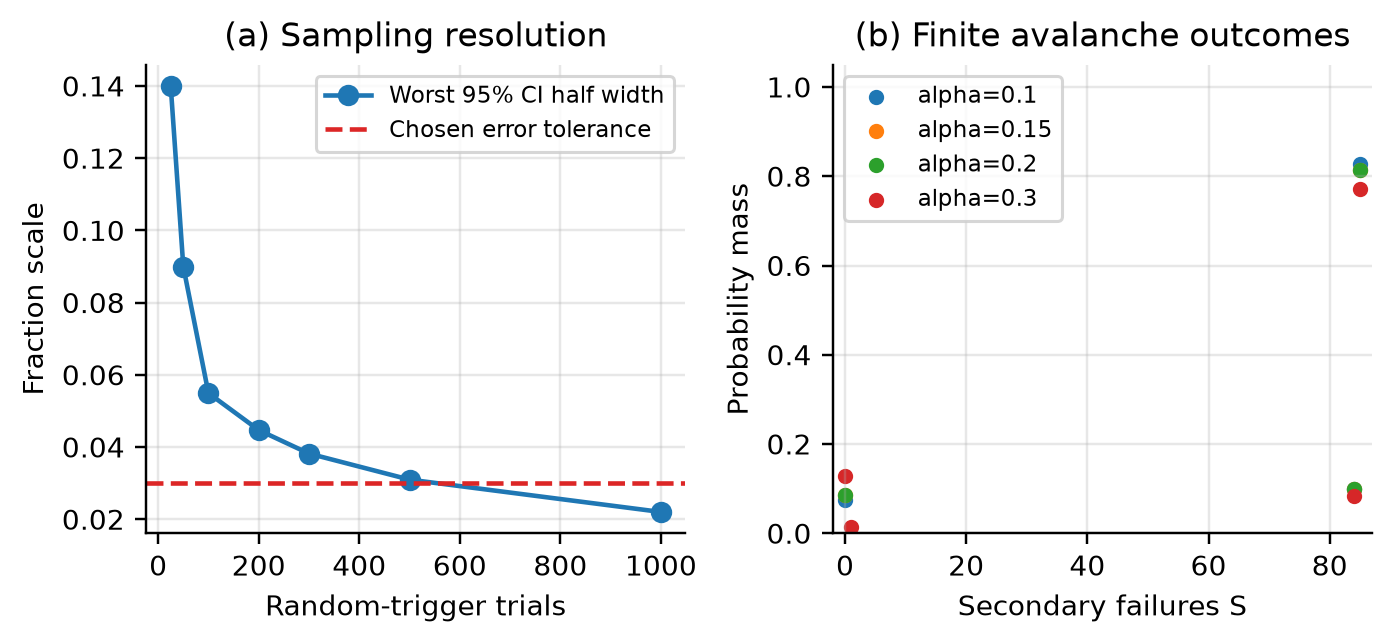
\includegraphics[width=\linewidth]{figures/uncertainty_avalanche.png}
  \caption{Uncertainty is conditional on the frozen graph and load model.
  (a) Worst pointwise 95\% interval half width over the tested conditions with
  a common available prefix size. The 0.03 line is a chosen numerical tolerance;
  the accompanying mean-change criterion is checked separately. (b) Static
  capacity-rule probability masses from 2,000 random triggers at each alpha;
  zero secondary failures remain in the denominator and alphas are not pooled.
  Most mass lies at a few finite sizes, unsuitable evidence for broad scaling.
  Sources: P2.5 recommendations and P2.2 avalanche samples.}
  \label{fig:uncertainty}
\end{figure}

\clearpage

% --- References (excluded from the five-page limit) -----------------------
\bibliographystyle{plainnat}
\bibliography{references}

% --- Appendices (excluded from the five-page limit) -----------------------
\appendix
\clearpage
% Appendix (excluded from the five-page limit).
% Use this for supplementary material such as extra parameter scans,
% derivations, or links to simulations and notebooks.

\section{Reproducibility and supplementary evidence}
\label{app:supplementary}

The repository is
\url{https://github.com/CITS4403-Project/Project}. The live demonstration uses
\path{notebooks/01_network.ipynb} and
\path{notebooks/03_cascades.ipynb}, alongside the P3.2/P3.4 notebooks.
These run from committed inputs and do not require a live timetable download.
Full model definitions and raw-feed reconstruction are in
\texttt{docs/model.md} and \texttt{docs/data.md}.

\begingroup
\raggedright
The RQ1 crossing table is \path{percolation_critical_fractions.csv} in
\path{results/percolation/}; susceptibility peaks and GCC crossings occupy
separate columns.
RQ2 uses \path{results/cascade/runs.csv} and
\path{avalanche_samples.csv}. RQ3 uses
\path{results/recovery/bus_cascade_scan.csv},
\path{bus_cascade_loads.csv} and
\path{strategy_comparison.csv}. RQ4 uses
\path{results/uncertainty/recommendations.json},
\path{power_law_fits.json} and
\path{results/demand/demand_alpha_star.csv}.
Every source has a metadata sidecar. The selected-figure manifest additionally
records table, sidecar, generator and output hashes.
\par\endgroup

From the repository root, \texttt{make figures} regenerates the three selected
images and the numeric macros used in the abstract and results. Then run
\texttt{make} inside \texttt{report/}, or use the documented Tectonic command in
\texttt{report/README.md}. The P2 runners
reproduce full experiments; the figure generator only reads their frozen
outputs. Bootstrap intervals quantify pointwise Monte Carlo error; they do
not cover different dates, measured demand or model misspecification.

\begin{table}[!ht]
  \centering
  \caption{Airport Line exclusive-station closure, $\alpha=0.2$. The policy
  budget is two selected links. Fractions use common intact denominators.}
  \label{tab:airport}
  \begin{tabular}{lrrr}
    \toprule
    Policy & Secondary closures & Served OD (\%) & Served weight (\%) \\
    \midrule
    No backup & 0 & \AirportRailServicePercent & \AirportRailDemandPercent \\
    Existing bus & 1 & \AirportBusServicePercent & \AirportBusDemandPercent \\
    \bottomrule
  \end{tabular}
\end{table}


\end{document}
